\chapter{GPU/CUDA并行原理和并行需要解决的问题}
\label{cha:chap03}


本章首先介绍GPU硬件结构、CUDA并行原理、以及本文使用到的CUDA性能优化技术,然后结合本文需要加速的算法对于可能遇到的加速难点进行了识别。本章对于实现一个并行算法不具有很大的意义,但是对于已经实现的高效的并行程序至关重要。

本章节的图~\ref{fig:GPU-HW-Arch}和图~\ref{fig:nvidia-cuda-arch}全部根据参考文献~\cite{nickolls2009graphics}和参考文献~\cite{lippert2009nvidia}绘制。本文介绍GPU硬件和CUDA相关技术都是以英伟达的GPU为例介绍的,对于其他GPU或者并行技术没有覆盖。

\section{GPU/CUDA并行原理}
\label{cha:chap03:gpu-HW-Arch}

GPU/CUDA并行是单指令多数据(Single Instruction Multiple Data,SIMD)并行方式的。SIMD并行是将数据元素映射到并行处理线程交由相同的程序处理。下面从GPU硬件架构和CUDA并行原理方面进行介绍,其中,GPU硬件结构部分介绍GPU的硬件结构组成来了解并行的基础,CUDA并行原理部分来说明CUDA如何使用GPU硬件完成并行任务的。

\subsection{GPU硬件结构}
%\label{}
图~\ref{fig:GPU-HW-Arch}介绍了GPU的典型硬件结构,GPU硬件包括了流处理器、流处理器簇、内存(全局、共享、常量等)几个关键部分。下面从这个几个主要部分的定义开始介绍GPU硬件结构。

\begin{figure}[H] % use float package if you want it here
	\centering
	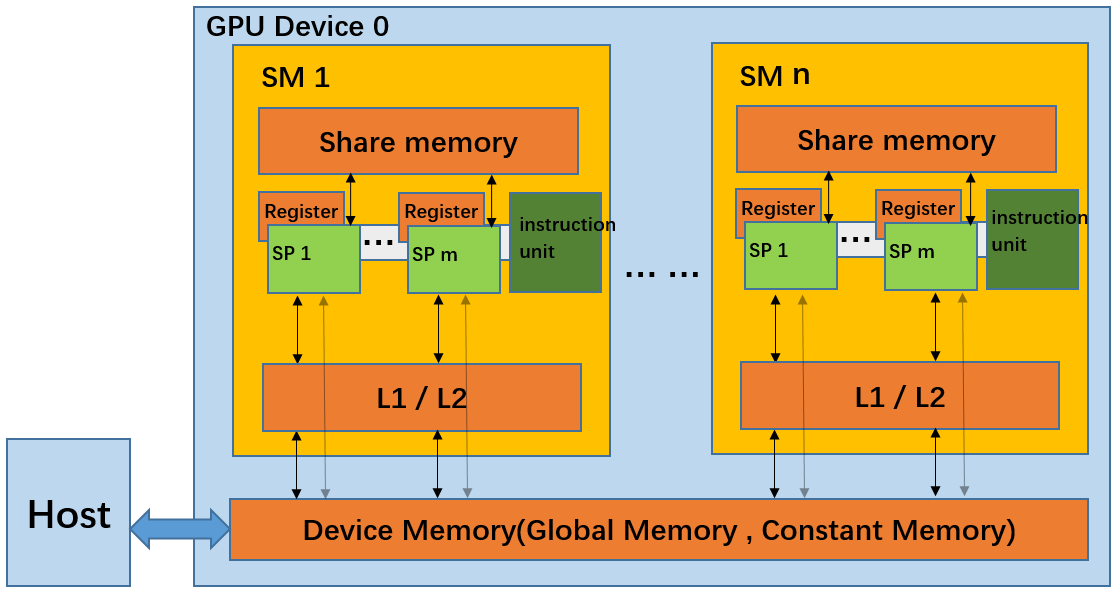
\includegraphics[height=6.2cm]{gpuarch.png}
	\caption{GPU硬件结构}
	\label{fig:GPU-HW-Arch}
\end{figure}

流处理器(Streaming Processor,SP)是GPU最基本的单元( 计算单元),承载一个线程的基本单元,SP又称为CUDA核,如图~\ref{fig:GPU-HW-Arch}的SP x。

流处理器簇(Stream Multiprocessors,SM)是由一定数量的SP加上指令单元、寄存器、共享内存、L1/L2缓存等组成。从图~\ref{fig:GPU-HW-Arch}可以看出,每个SM是由多个SP和一个指令单元组成,SM本身就是一个SIMD处理单元。

GPU实际上是一个SM的阵列,而SM又是由多个SP组成,GPU进行并行计算的本质就是众多SP共同进行数据计算。以GTX-1080来讲,GPU含有20个SM,每个SM含有128个SP,即在GPU最多可以同时运行$20*128$个线程。

全局内存(Global  memory)是独立于GPU内核的内存,而又是空间最大的内存,但访问延时最长。如图~\ref{fig:GPU-HW-Arch}所示,全局内存有以下特点:对于所有SP可见( 所有SP都可以读写全局内存);可以通过和主存建立主机和GPU之间的数据通信;两个并行任务之间的中间结果必须使用全局内存来处理。

共享内存(Share memory),是存在SM内部可以由SM内部多个线程共享使用的内存,速度是全局内存的几百倍。可以通过共享内存完成协作计算。

寄存器(Registers)是GPU中最快的内存,用于存储线程中的临时变量,只在线程内部可见。

本地内存(Local memory)是存储堆栈中无法容纳的所有内容的寄存器,本地内存存储在全局内存中,对于线程可见。

常量内存和纹理内存在本文中没有使用,在这里不做介绍。

表~\ref{tab:memory}对于使用到的内存的性能进行比较,更好的理解各内存在程序中所起的功能。

\begin{table}[htbp]
	\centering
	\begin{minipage}{0.7\textwidth}
		\caption{GPU内存比较}
		\label{tab:memory}
		\begin{tabular}{p{2cm}p{2cm}p{2cm}p{2cm}p{2cm}}
			\toprule[1.5pt]
			{\heiti 内存} & {\heiti 速度}(周期)&{\heiti 大小} &{\heiti 范围} &{\heiti 周期}\\\midrule[1pt]
			全局内存 & $\sim$400-600 & 8G & Grid & The whole procedure \\
			共享内存 & $\sim$20 & 48K(每个Block) & Block & thread \\
			寄存器 & $\sim$1 & 64K(每个Block) & thread & thread \\
			\bottomrule[1.5pt]
		\end{tabular}
		
	\end{minipage}
\end{table}

\subsection{CUDA并行原理}

前面从硬件角度介绍GPU的硬件结构,本章节将从软件角度叙述CUDA如何利用GPU的硬件基础进行并行计算的,首先介绍几个CUDA的基本概念。

线程(Thread)是并行程序的基本单元,一个并行程序是由很多线程共同执行,图~\ref{fig:nvidia-cuda-arch}带箭头的曲线表示一个线程。

线程块(Block)由多个线程组成,在一个Block中线程可以进行同步( 需要通过程序控制),也可以通过共享内存进行通信。 图~\ref{fig:nvidia-cuda-arch}的Block(x,y)表示线程块,这里的线程块是由多个线程以阵列形式组成。

线程束(Warp),将Block连续线程ID聚合起来的32个线程(比如thread 0~31,32~63)定义为一个Warp,Warp是调度和运行的基本单元,Warp中所有线程并行的执行相同的指令并且是严格同步的,这中同步是由硬件底层完成而不需要通过程序来控制。将一个Block连续的32个线程聚合成一个Warp,当一个Block的线程个数不是32个整数倍时,硬件会帮助凑足32个线程形成一个Warp,这样就会造成资源的浪费。因为SM是一个SIMD处理器,要求所有线程执行相同的指令,如果遇到分支语句,将会将两个分支串行执行。

线程网格(Grid),多个Block构成线程网格,Grid是程序调度的接口。图~\ref{fig:nvidia-cuda-arch}的Grid 1是由6个Block组成。

\begin{figure}[H] % use float package if you want it here
	\centering
	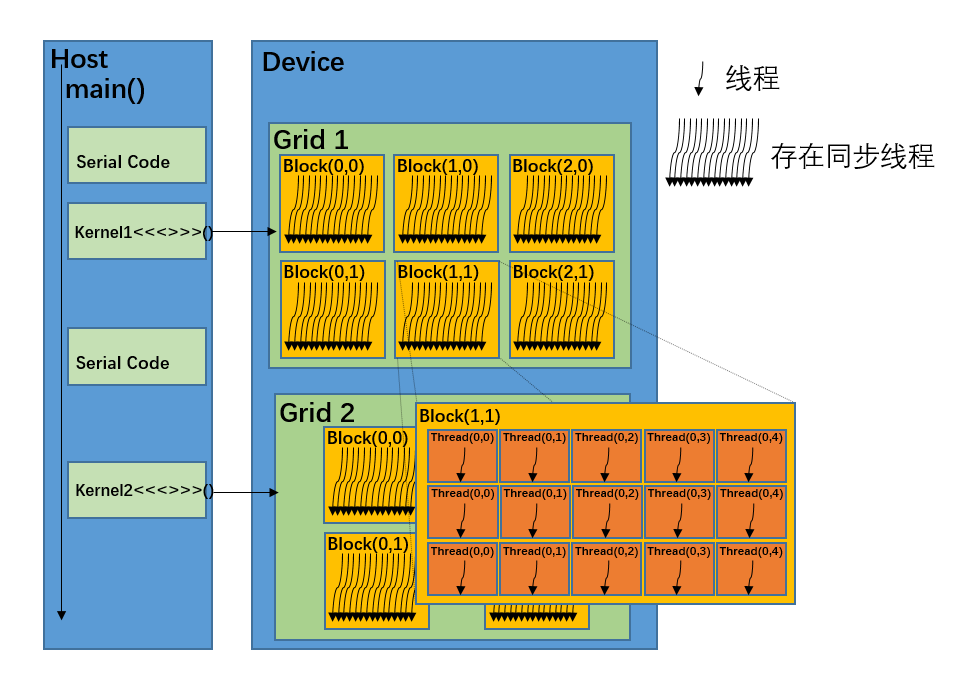
\includegraphics[height=7.5cm]{kernelexcute.png}
	\caption{NVIDIA CUDA架构}
	\label{fig:nvidia-cuda-arch}
\end{figure}

以GTX 1080为例,一个Grid最多可以有$2^{31}-1$个Block,一个Block最多可以有1024个线程,但是在硬件上每个GPU只有20个SM,每个SM只有128个。正常情况下2560个SP是不能运行这么多线程的。

一个SP可以执行一个线程,但是实际上并不是所有的线程能够在同一时刻执行,GPU运行线程也是采用了分时复用的思想。英伟达把连续的32个线程组成一个Warp,最多1024个线程分成32个Warp。而GTX 1080一个SM有4个Warp调度单元,可以同时容纳4个Warp运行。起初所有Warp都在就绪队列中,首先从就绪对列取出4个Warp在SM上执行,当某个Warp因为读取内存操作而挂起时,Warp调度单元从就绪队列取出一个Warp执行;当正在内存请求的Warp完成内存请求之后,线程束将会进入就绪状态。

多个Warp在4个Warp调度单元通过分时复用的方式进行并行运行,同理大量的Block在20个SM中运行的原理是一致的,都是利用计算资源分时复用的方法。CUDA并行是由成千上万的线程并行完成的,这些线程在软件层面是同时并行的,但是在物理层面最多只有2560个线程在运行,其他都在挂起或者就绪状态。

\section{CUDA相关技术}
章节~\ref{cha:chap03:gpu-HW-Arch}介绍GPU/CUDA的并行原理,本章在并行原理的基础上介绍后文用到的CUDA加速技术,包括合并存储器访问、隐藏延时等。

\subsection{合并存储器访问}

从表~\ref{tab:memory}可以看出访问全局内存是内存访问耗时最长的环节,但全局内存又是GPU内存最大的部分,当处理大量数据的并行时,不可避免会存在大量的全局内存读写操作,这样全局内存访问有可能称为性能优化的瓶颈。这里可以通过合并存储访问来优化全局内存访问性能。

合并存储器访问( Coalesced Memory Access),是当特定的访问条件满足时,设备将一个Warp内线程的全局读写操作合并成一个事务。这里特定的条件是一个Warp内线程访问连续的128K空间,而且线程和128K的地址一一对应( 但不要求严格对齐),如图~\ref{fig:coalesced}~\cite{woolley2013gpu}。一个Warp中32个线程只需要经过一次L1缓存的过程,大大地提高了全局内存访问速度。

\begin{figure}[H] % use float package if you want it here
	\centering
	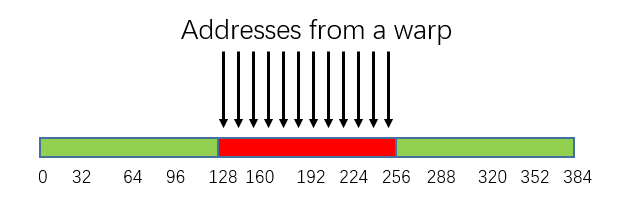
\includegraphics[height=2.5cm]{coaleced.png}
	\caption{全局内存合并访问示意图}
	\label{fig:coalesced}
\end{figure}

合并存储器访问加速全局内存访问可以通过Cache命中观点来解释:当一个Warp的32线程同时读写连续的128K空间,以某个线程首先读取了这个128K空间,设备(GPU中L1缓存的大小为128K)将这连续的128K空间缓存到L1 Cache中,其他31个线程再读写这个128K时,可以直接命中到Cache上读写( Cache的访问时延远小于全局内存),不需要经过内存读写挂起的过程,降低了访问时延。

另外,合并存储器访问经常和共享内存一起使用,因为共享内存是Block内部可见的,一个Warp中的线程从全局内存读取连续空间到共享内存,在共享内存完成复杂操作( 比如矩阵转置),然后在共享内存内容写入全局内存连续空间。


\subsection{延时隐藏}

线程不可避免会出现访问各种内存而产生额外的访存延时,为了使访存延时不影响执行速度,可以使用隐藏延时的方法来解决。SM使通过调度Warp来执行线程,可以通过增加Warp的个数来使Warp调度单元尽可能原则已经就绪的Warp,避免选择正在因为延时而挂起的Warp。将通过执行多个Warp来获取较高吞吐量的方法称为隐藏延时。

对于这种性能度量通常通过占用率来评价,占用率通过并行执行的Warp数量除以并发运行的最大可能Warp数量。高占用率意味着Warp调度器有很多Warp可供选择,能够隐藏延时访存等。

{\color{red}{按照下面方法计算占有率,这个得做实验}}
%较高的占用率并不总是等同于较高的性能 - 有一点超出额外占用率不会提高性能。 但是,低占用率总是会干扰隐藏内存延迟的能力,从而导致性能下降。在于评价?
%http://docs.nvidia.com/cuda/cuda-c-best-practices-guide/index.html#memory-optimizations    Execution Configuration Optimizations
%尽量增加SM上的线程数量,提高Occupancy(实际并发运行的warp个数/最大可能并发运行的warp个数);
%http://blog.163.com/wujiaxing009@126/blog/static/71988399201709105252458/
%a. 限制条件:# of registers和# of shared memory, 一个SM可以并行处理768 threads
%b. 100%Occupancy: 2 blocks X 384 threads
%3 blocks X 256 threads
%4 blocks X 192 threads
%6 blocks X 128 threads
%8 blocks X 96 threads
%c. 最小存储器延时:Occupancy≥50% and threads/blocks≥128
%(2) Thread block内的线程个数应该是warp size的整数倍,避免在一个warp内有分支语句;
%(3) Grid/Block Size Heuristics;
%a. # of blocks / # of SMs > 1
%每个SM至少有一个thread block可以执行
%b. 更好的选择:# of blocks / # of SMs > 2
%每个SM有多个thread block可以执行
%c. 每个block占用SM一半以下的资源
%d. # of blocks > 100 使得适应将来的结构

%线程指令是在CUDA中顺序执行的,因此,当一个warp暂停或停顿时执行其他warp是隐藏延迟和保持硬件繁忙的唯一方法。 因此,在确定硬件保持繁忙的有效程度时,与多处理器上的活动warp数相关的一些度量标准非常重要。 这个度量是占用率

\subsection{关于Warp的注意事项}

因为Warp使GPU调度得基本单元,每个SM又是SIMT处理器(只有一个指令单元),因此Warp内的线程只能执行同一条指令,当遇到分支语句时,不同的线程可能执行不同的语句,这和Warp内线程只能执行一个指令矛盾。分支语句会被序列化,一个Warp中只能执行一个分支即部分线程执行,其他分支的线程都处于挂起状态,这样会导致性能的降低,这种现象称为Warp分歧(Warp divergence)。为了避免Warp分歧现象,尽量避免同一个Warp存在不同的分支路径。

{\color{red}{序列化这个东西是编译器处理还是CUDA执行单元处理的}}

\subsection{共享内存使用和存储器冲突}

前面提到共享内存,相比全局内存拥有更小的时延和更高的带宽,并且线程之间可以通过共享内存进行通信和协作计算,但是使用共享内存有一个前提条件:不能出现存储器冲突(Bank Conflict)。

共享内存实际上是以4bytes为单位分为多个存储体(Bank),以GTX 1080为例 $\_\_share\_\_ int\quad data[128]$,假设,那么$data[0]$属于Bank0,$data[1]$属于Bank1,...,$data[31]$属于Bank31,...。当出现一个Warp内的两个线程访问一个bank的两个元素时,同一个Bank的访问请求就会被序列化,会造成多倍的访问延时。

这里有一个特殊情况,当一个Warp内的所有线程访问一个存储器中的同一个地址时,共享内存会将这个地址下的数据广播到Warp所有线程中。

{\color{red}{检查一下代码有没有这样的问题,通过下面这个地址自查一下}}
%https://blog.csdn.net/Bruce_0712/article/details/65447608
\section{GPU并行可能遇到的问题}

\subsection{数据集不断增大的问题}
\label{cha:chap03:Problemsencountered:BigDataSet}

$\mathcal{F}$是计算Shapelet中一个空间复杂度为$O(N)$的中间变量,是计算距离和最佳分割点的中间变量。当N很小的时候,我们采用寄存器存储$\mathcal{F}$,速度不会受影响;当N增大时,CUDA会将寄存器存不下的内容放在局部内存中(局部内存实际上占用全局内存空间,和全局存储速度一致,但是又没有使用全局内存合并访问),因此性能比较差。

这里提出将$\mathcal{F}$放在全局内存中存储作为计算距离和最佳分割点的中间变量,而计算距离和最佳分割点分别作为线程读写$\mathcal{F}$,其中两阶段都是用全局合并访问的方法访问$\mathcal{F}$。

当数据集不断增大时(即N,L不断增大),中间结果一共有$O(NL^2)$个$\mathcal{F}$,空间复杂度为$O(N^2L^2)$。因为全局内存是有限的,$O(N^2L^2)$的空间复杂度很快会使内存超过全局内存大小。对于全局内存相对于中间结果不足的情况,这里使用换入换出的思路去解决,每次对于$SubSet(D)$的子集计算$g(D,(Shapelet(D),d_{osp(Shapelet(D))}))$,综合多次结果。

\begin{definition}
	\label{def:chap03:Threephases}
	Shapelet并行过程三阶段:本文将Shapelet计算过程分为三个阶段,分别为距离计算阶段、最佳分割点计算阶段、求最大信息增益阶段。其中距离计算阶段是指从候选序列$S$和数据集$D$到$S$相对数据集$D$距离-类标对集合$\mathcal{F}$的过程;最佳分割点计算阶段是指从$\mathcal{F}$到$S$对应的最佳分割点$d_{osp(S)}$以及对应的信息增益的过程;求最大信息增益阶段是指从并行获得的多个信息增益到最大信息增益以及对应的候选序列和分割点的过程。
	
	这里,章节~\ref{cha:chap03:Problemsencountered:BigDataSet}解释了为什么从$\mathcal{F}$出分成两个阶段;至于从最佳分割点计算处分为两个阶段的原因,并行计算最佳分割点,必然产生多个信息增益,当数据集很大时,就有必要对于多个信息增益求最大值的过程进行并行,所以有了求最大信息增益
\end{definition}


\subsection{优化困难}

上面提到实现一个并行程序不是很难,但是使并行程序表现出很好的性能需要消耗大量的时间。

比如grid参数考虑



